% different platforms
  % 1G
  % 10G
  % SUME
  % CIVIL
  % pros and cons
% Why NetFPGA
% What does NetFPGA provide
% standalone and integrated


The \textit{NetFPGA} platform is an ``open source hardware and software platform designed for research and teaching'' \cite{NetFPGA}.
\textit{NetFPGA} provides four hardware platforms, each with a different specification and target audience. As decribed in the initial specification in appendix \ref{initial_spec}, the \textit{NetFPGA 1G} was initially considered to be the most suitable hardware platform for this project, due to its compatibility with general purpose consumer hardware.
This was in part due to its use of UTP copper, while all other \textit{NetFPGA} platforms use fibre optics.

While the \textit{NetFPGA 1G} would have been the most suitable hardware platform for a prototype model, this prototype is no longer being developed due to a change in the focus of the project, and the most suitable hardware platform for a production model would be the \textit{NetFPGA SUME} (shown in figure \ref{netfpga_sume_figure}). This platform is based around a \textit{Xilinx Virtex-7 690T} \cite{virtex7-690t} which contains 693,120 logic cells and 52,920 Kbit block RAM. It also incorporates 10-Gigabit Ethernet networking ports, as well as 4 external SFP+ ports for connections of up to 100Gbps. Just like the \textit{NetFPGA 1G}, it has a standard PCI form factor, and so is compatible with most consumer motherboards as an add-on card, or can also be used as a standalone board.

% Of the four hardware plaforms available, the NetFPGA 1G \cite{NetFPGA_1G} is the most suitable for this project, since its hardware is most compatible with general purpose consumer hardware. The other three platforms could be used to create faster circuits than the NetFPGA 1G, but these may require additional hardware, which is not currently available for this project. This platform is based around a \textit{Xilinx Virtex-II Pro 50} \cite{virtex2-pro} which contains 53,136 logic cells and 4kb block RAM. In addition, the NetFPGA 1G contains four Gigabit Ethernet networking ports, 4.5MB of SRAM, and 64MB of DDR2 DRAM. It has a standard PCI form factor, and so is compatible with most consumer motherboards.

\begin{figure}[t]
  \centering
  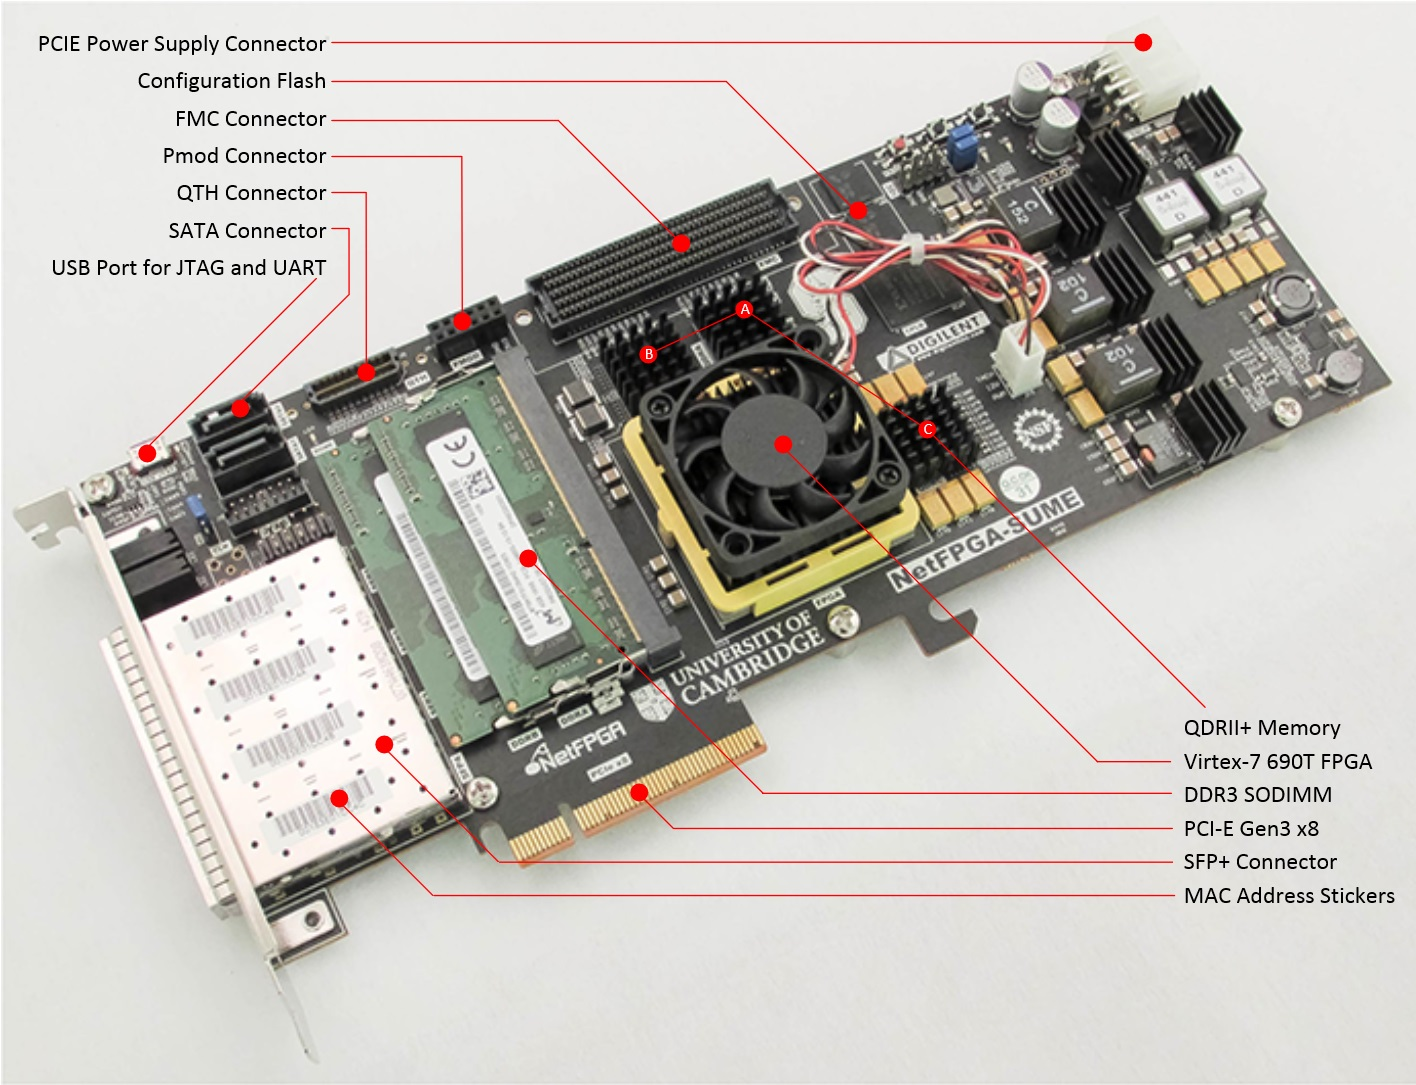
\includegraphics[width=\textwidth]{assets/netfpga_sume.jpg}
  \caption{Labelled NetFPGA SUME}
  \label{netfpga_sume_figure}
\end{figure}

% From spec
% The NetFPGA \cite{NetFPGA} platform is intended to be used for this project. It is an ``open source hardware and software platform designed for research and teaching'' \cite{NetFPGA_about}. Of the four hardware plaforms available, the NetFPGA 1G \cite{NetFPGA_1G} is the most suitable for this project, since its hardware is most compatible with general purpose consumer hardware. The other three platforms could be used to create faster circuits than the NetFPGA 1G, but these may require additional hardware, which is not currently available for this project. This platform is based around a \textit{Xilinx Virtex-II Pro 50} \cite{virtex2-pro} which contains 53,136 logic cells and 4kb block RAM. In addition, the NetFPGA 1G contains four Gigabit Ethernet networking ports, 4.5MB of SRAM, and 64MB of DDR2 DRAM. It has a standard PCI form factor, and so is compatible with most consumer motherboards.
